\documentclass{article}
\usepackage{graphicx} %package to manage images
\usepackage[utf8]{inputenc}
\usepackage[a4paper, total={6in, 8in}]{geometry}
\usepackage{xurl}
\usepackage{float}
\title{Relatório 11 \\ Análise das fixações}
\author{Pedro A. S. O. Neto}
\date{Julho, 2022}

\begin{document}

\maketitle

\section{Tempo total de fixação}

Calcula-se o tempo total de fixação em cada parte da tela (Rosto, Direita, Esquerda), durante cada condição (RJA, IJA), e foco de brinquedo (Direita, Esquerda).

Exemplo de como ler os gráficos abaixo: para videos IJA, as crianças passam mais tempo olhando para os objetos de interesse do que para os objetos distratores (Direita ou esquerda). Essa relação não é tão forte para vídeos RJA.

\begin{figure}[]
\caption{Tempo total de fixação. Pontos pretos indicam outliers.}
\noindent\makebox[\textwidth]{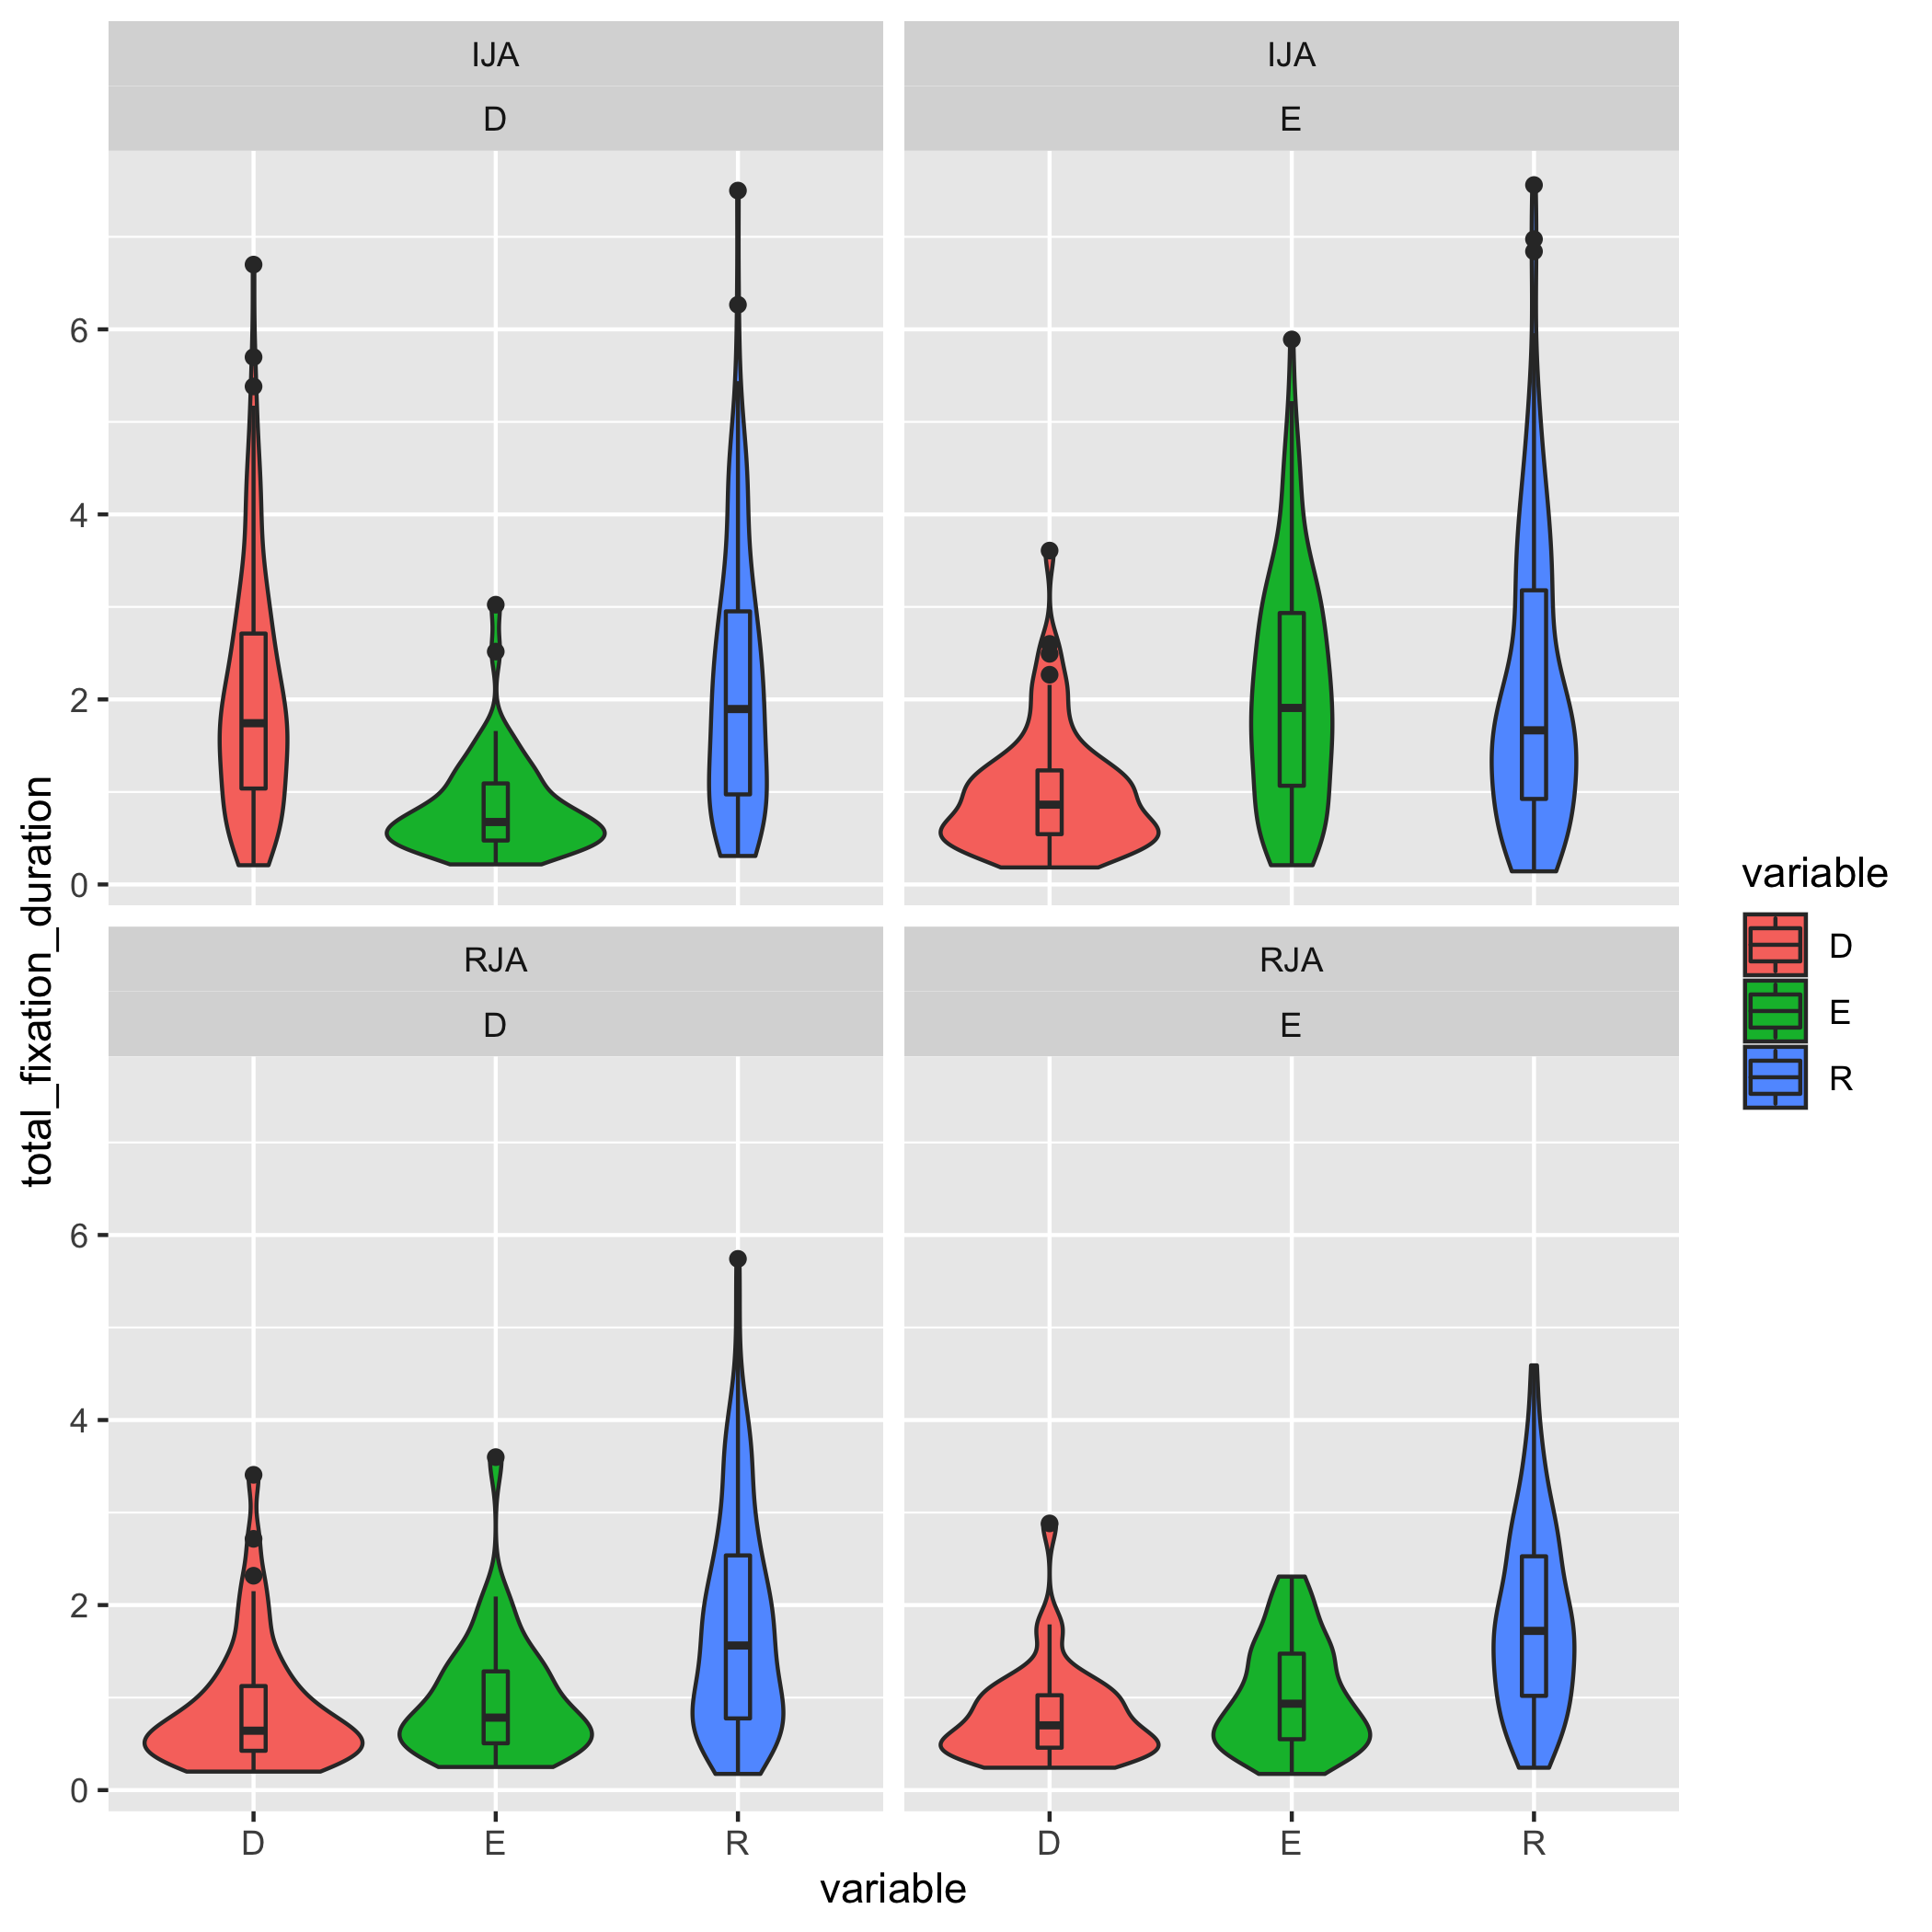
\includegraphics[scale=0.2]{"./totalFixationDuration.png"}}
\centering
\end{figure}

\begin{figure}[]
\caption{Tempo total de fixação. Pontos pretos indicam outliers.}
\noindent\makebox[\textwidth]{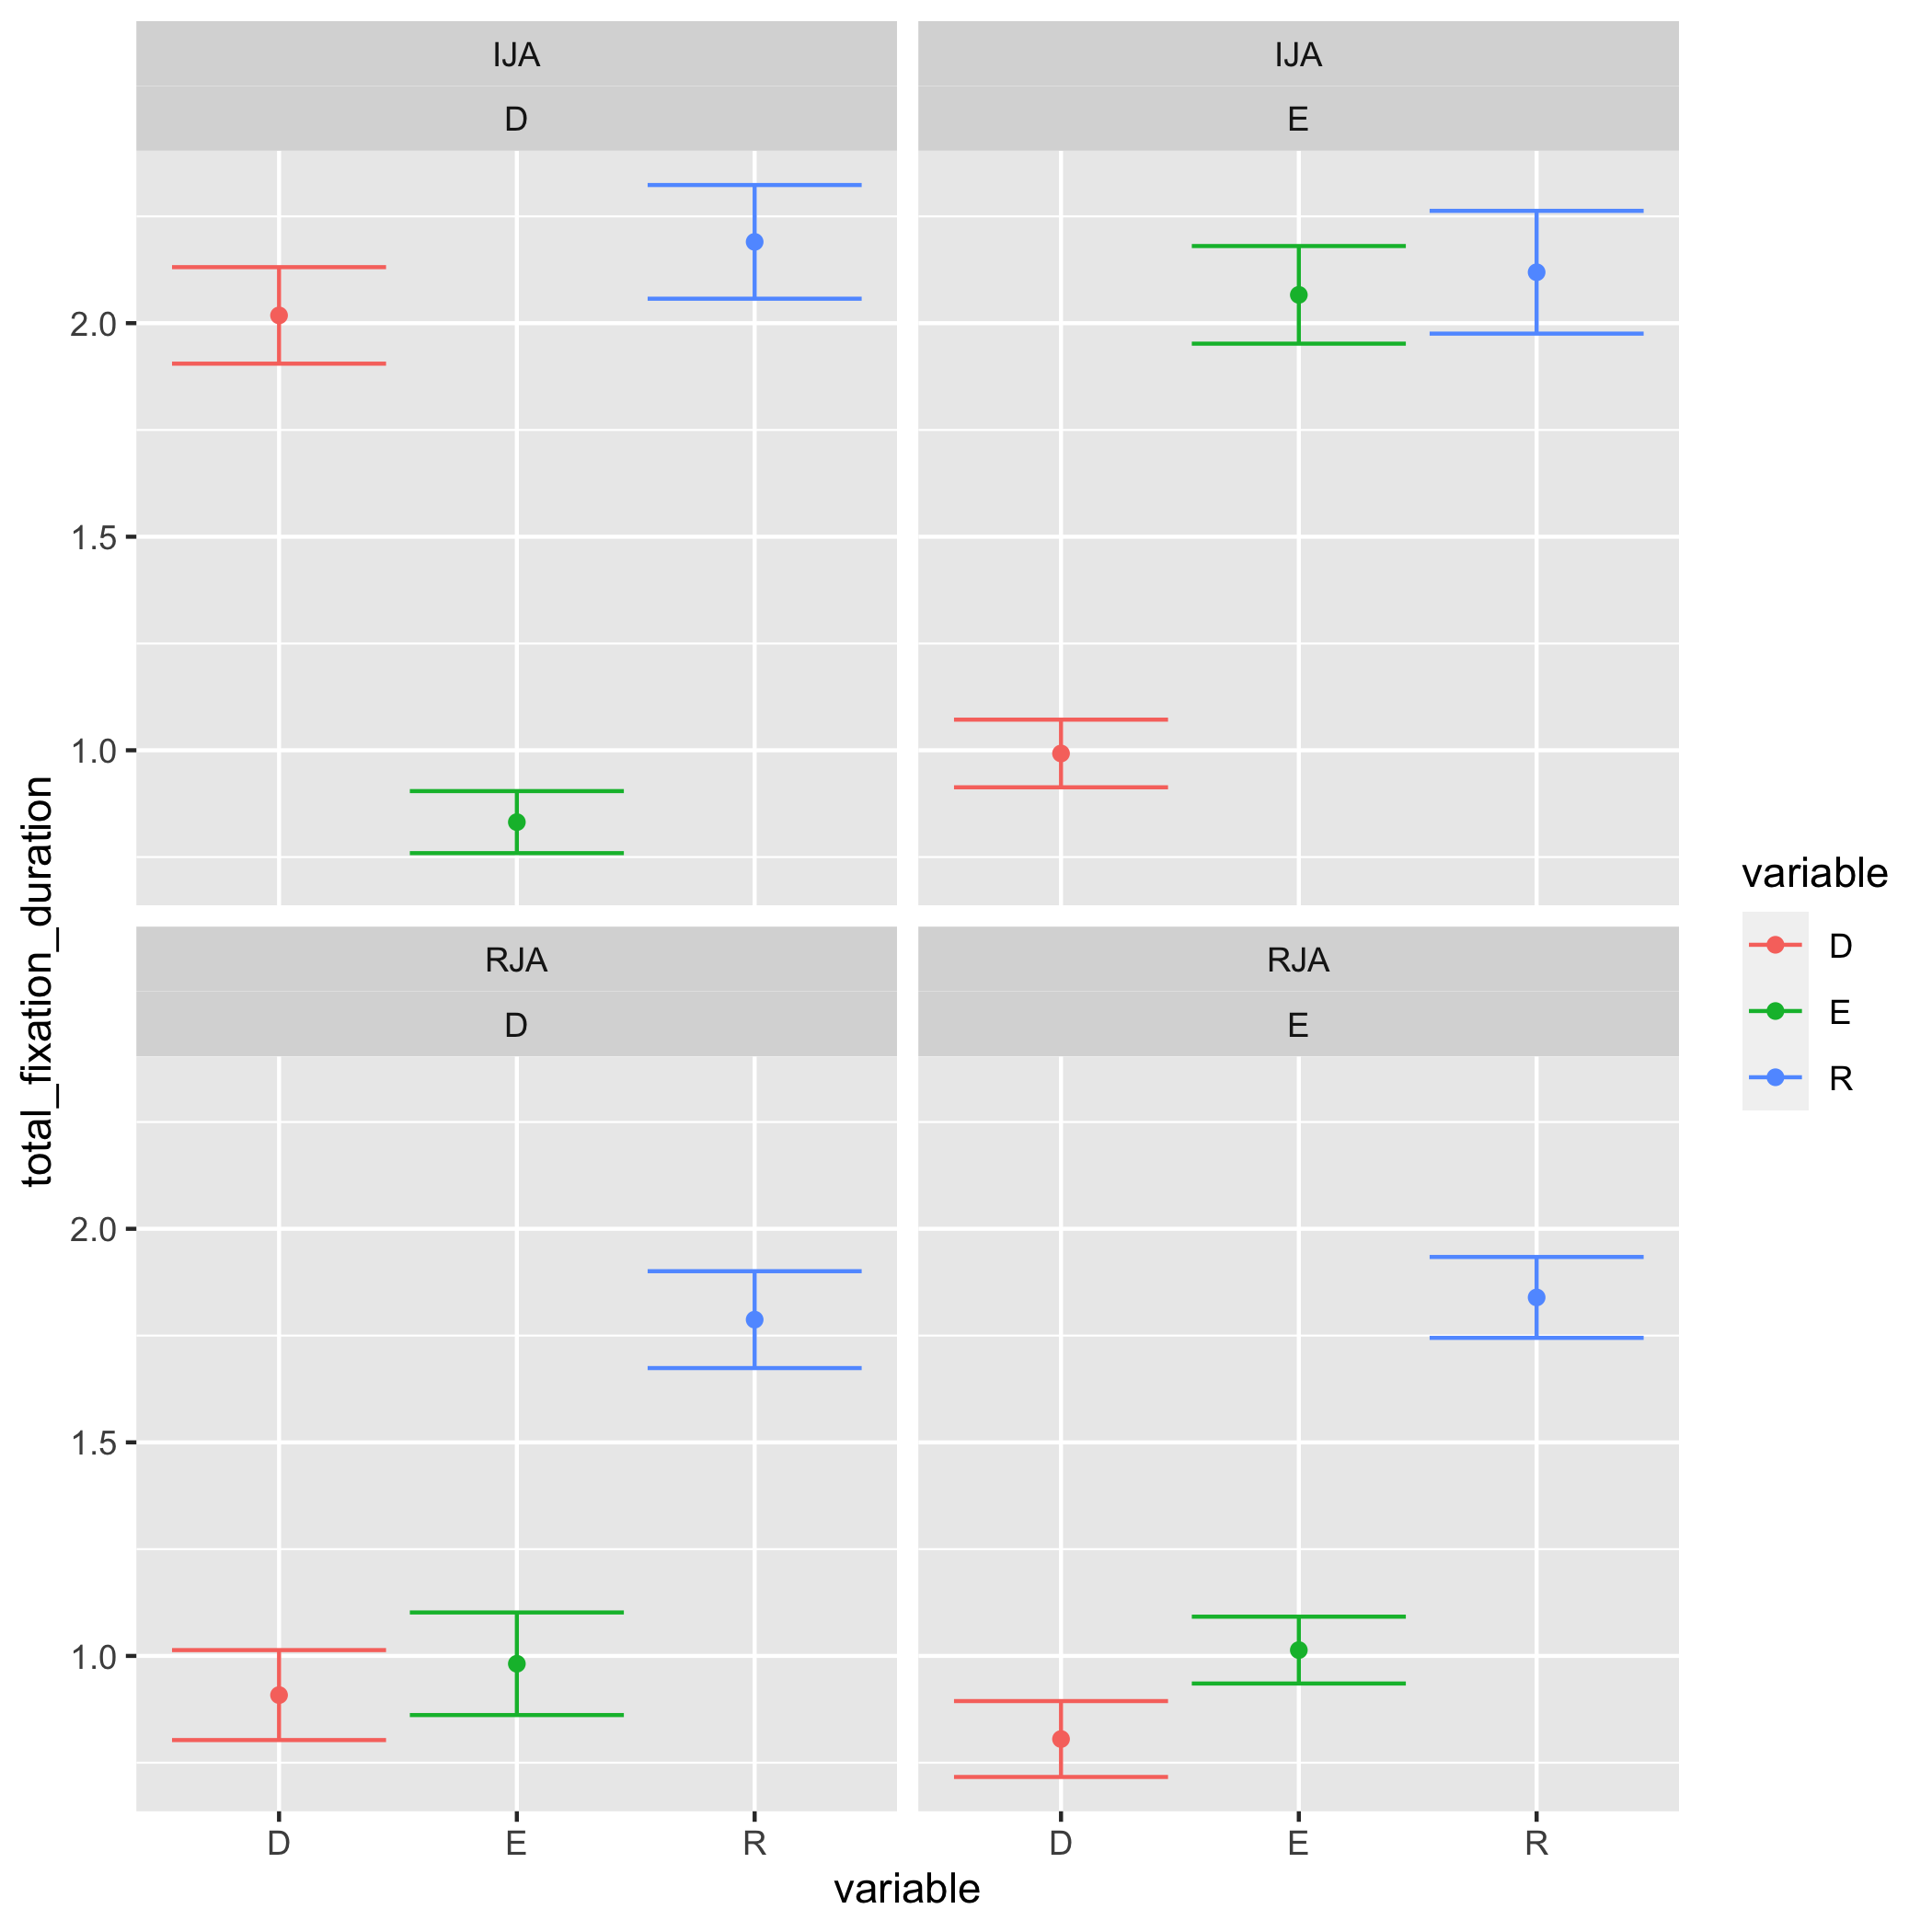
\includegraphics[scale=0.2]{"./totalFixationDuration2.png"}}
\centering
\end{figure}

\section{Index e contagem de fixação}

Calcula-se o index de fixação de acordo com a fórmula $(c-e)/t$, onde $c$ indica o número de fixações no objeto correto (Direita ou Esquerda), $e$ indica o número de fixações no objeto errado, e $t$ o número total de fixações. O index vai de $-1$ a $1$. Quanto maior o valor, melhor é a performance do indivíduo.

\begin{figure}[]
\caption{Index de fixações para todos os participantes, por condição.}
\noindent\makebox[\textwidth]{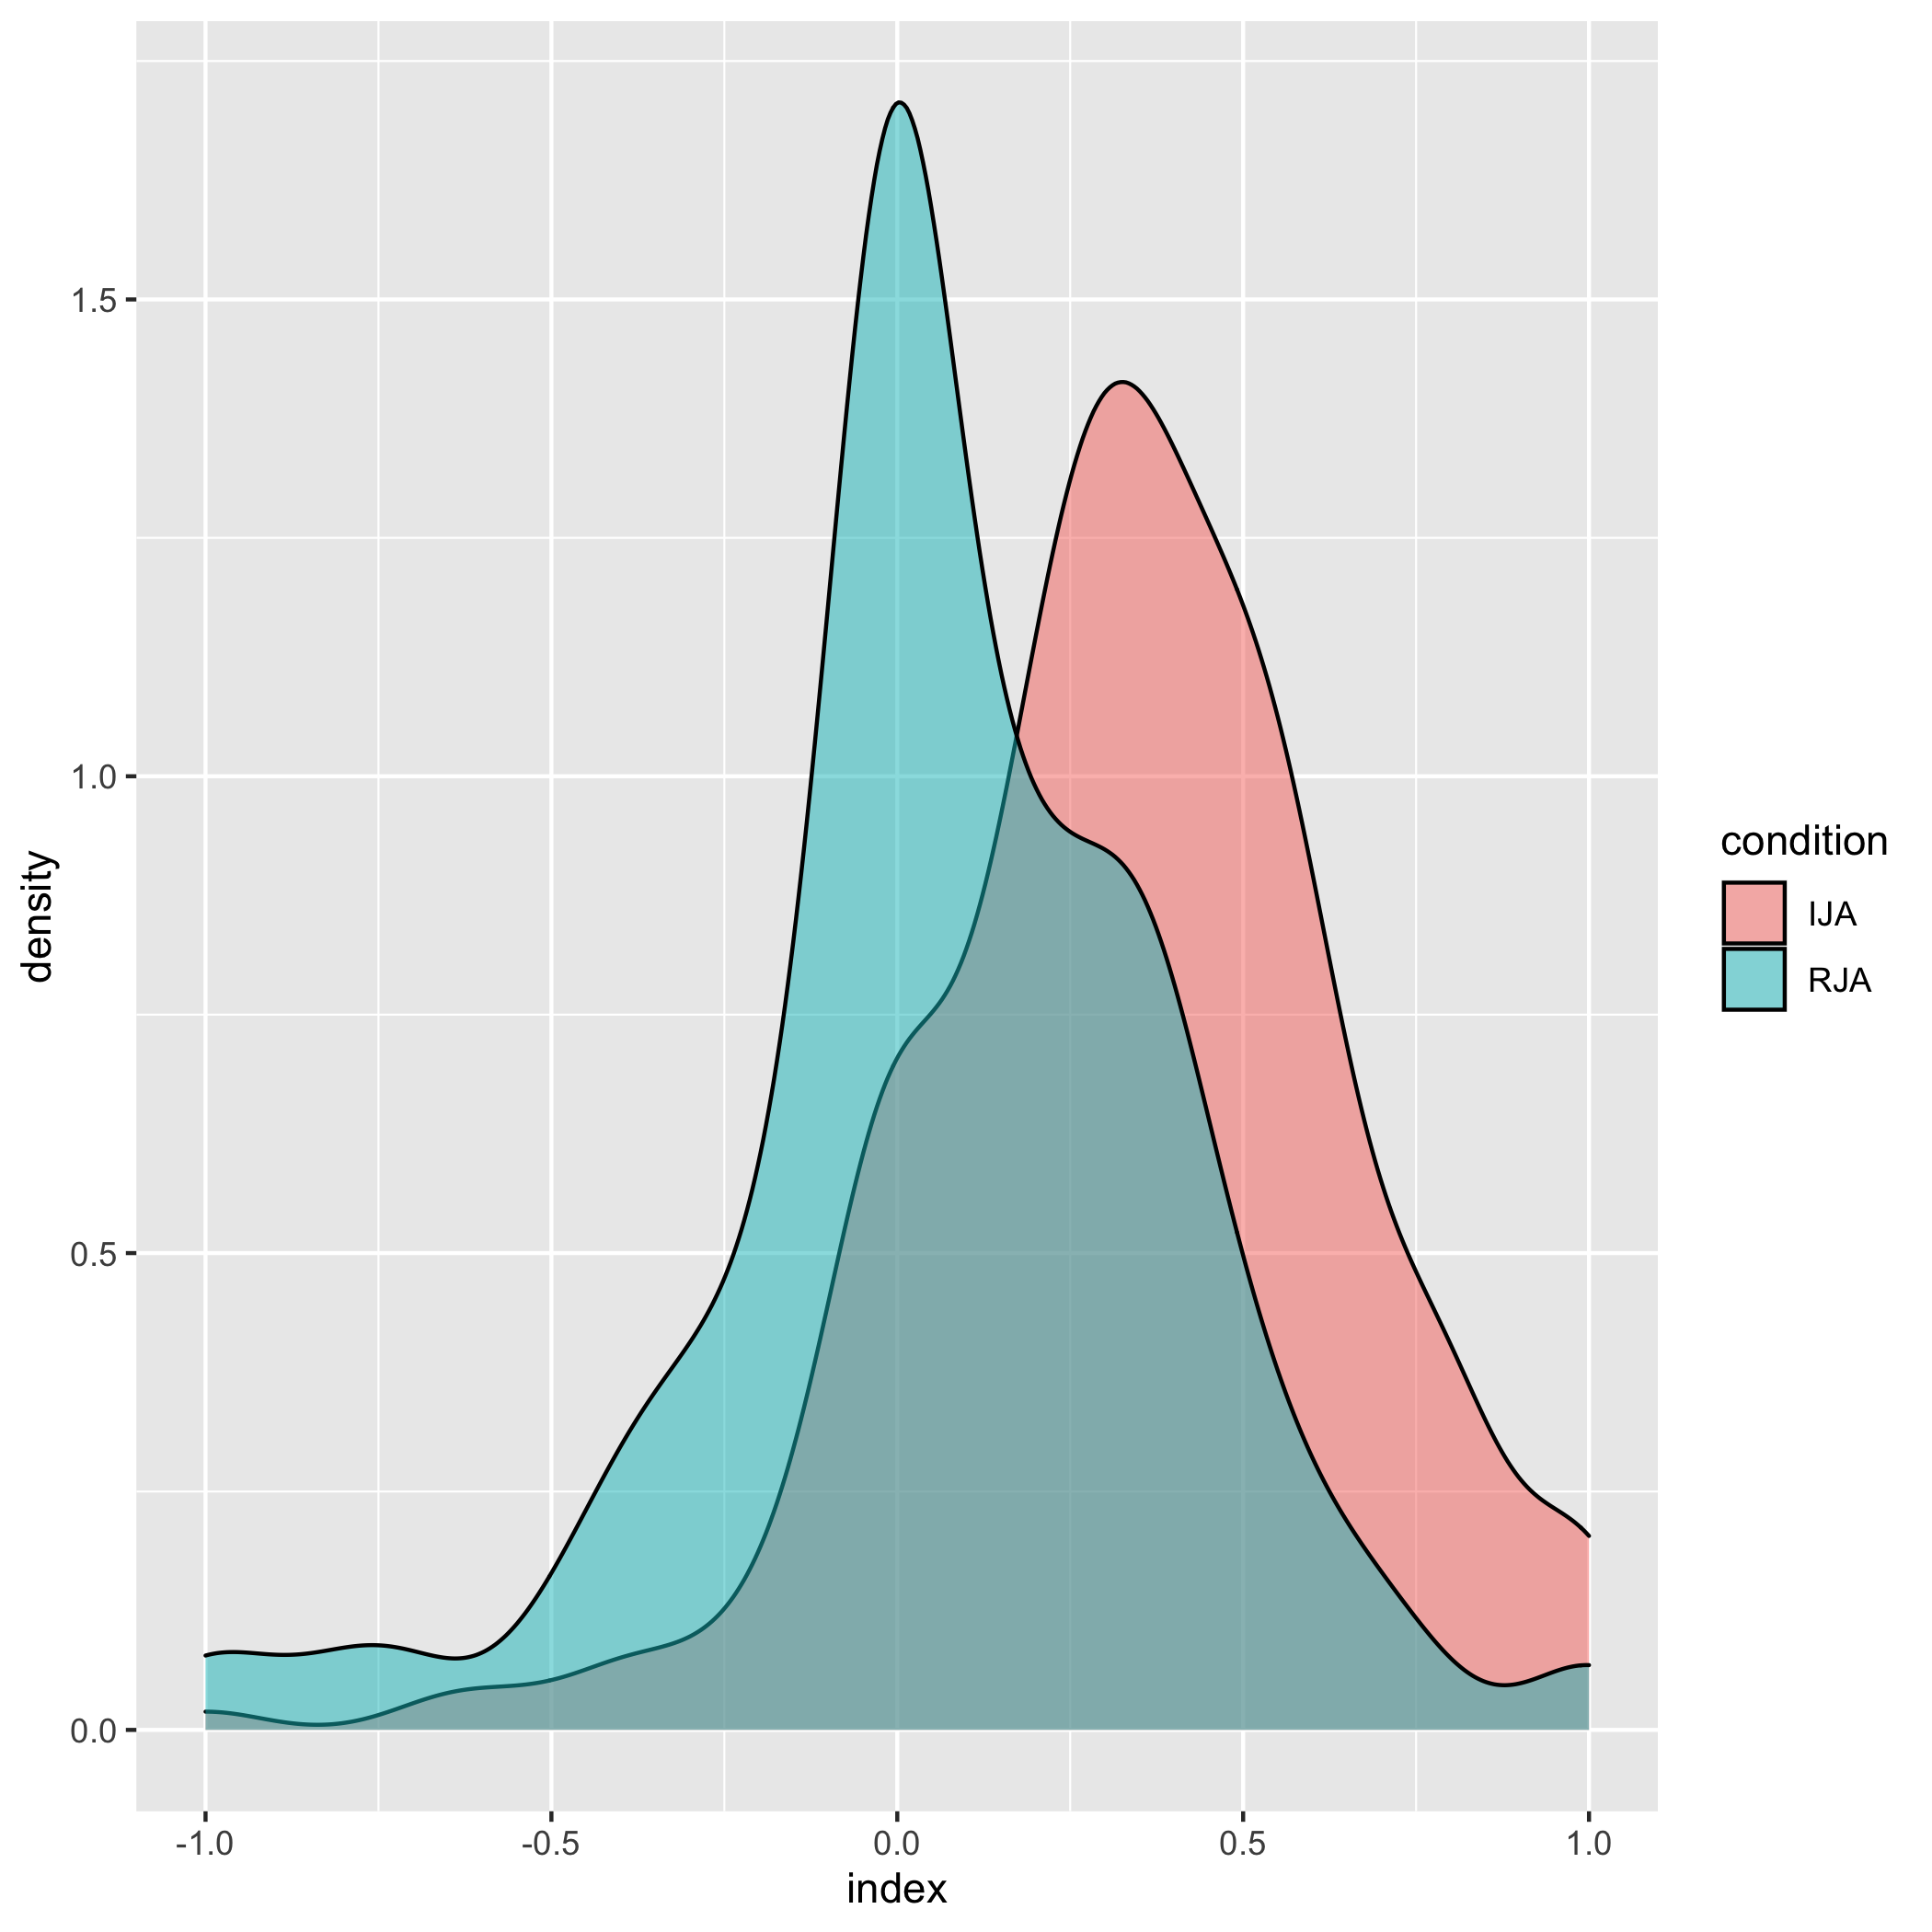
\includegraphics[scale=0.2]{"./countIndex.png"}}
\centering
\end{figure}

\end{document}
